
\PassOptionsToPackage{full}{textcomp}
\documentclass[]{tufte-handout}
%\usepackage{fontspec}
%\usepackage{ETbb}


% load babel package and options here
%\usepackage[p,osf]{ETbb} % osf in text, tabular lining figures in math
\usepackage{ETbb} % osf in text, tabular lining figures in math
\usepackage[scaled=.95,type1]{cabin} % sans serif in style of Gill Sans
\usepackage[varqu,varl]{zi4}% inconsolata typewriter
\usepackage[T1]{fontenc} % LY1 also works
\usepackage[libertine,vvarbb]{newtxmath}
%\usepackage[cal=boondoxo,bb=boondox,frak=boondox]{mathalfa}

%\geometry{showframe} % display margins for debugging page layout

\usepackage{graphicx} % allow embedded images
%  \setkeys{Gin}{width=\linewidth,totalheight=\textheight,keepaspectratio}
  \graphicspath{{graphics/}} % set of paths to search for images
\usepackage{amsmath}  % extended mathematics
\usepackage{booktabs} % book-quality tables
%\usepackage{units}    % non-stacked fractions and better unit spacing
\usepackage{multicol} % multiple column layout facilities
\usepackage{multirow} % multiple column layout facilities
\usepackage{lipsum}   % filler text
\usepackage{fancyvrb} % extended verbatim environments
  \fvset{fontsize=\normalsize}% default font size for fancy-verbatim environments
\usepackage{gensymb} % provides symbols like \degree
\usepackage{ragged2e} % enables hyphenation in ragged-right justification
\usepackage[normalize-symbols]{textalpha} %enables \textalpha for alpha symbol etc.

\usepackage{hyperref} % enables styling of href and url
\hypersetup{
    pdftitle={Tutorial X},
    pdfauthor={Barry Linkletter},
    colorlinks=true,
    linkcolor=blue,
    filecolor=magenta,      
    urlcolor=blue,
    pdfborder={0 0 0},
    frenchlinks=false,
    pdfpagemode=FullScreen,
    }

\usepackage{enumitem} % allows resuming enumerate lists.
\usepackage{mathtools}
\usepackage{mhchem}

\usepackage{siunitx} % provides "S" column class for aligning decimals.  


\usepackage{nicefrac}

\usepackage{varioref}

\usepackage{babel}
\usepackage{float}
\usepackage{stackrel}


\usepackage[shortconst]{physconst}

\usepackage[normalem]{ulem}  % provides strikethrough \sout{}

\usepackage{newfloat}
\DeclareFloatingEnvironment[
  fileext = los ,
  listname = {List of Schemes} ,
  name = Scheme
]{scheme}                    % provides scheme numbering for chemical schemes



\newcommand{\Km}{$\rm K_M$}
\newcommand{\Vmax}{$\rm V_{max}$}
\newcommand{\kcat}{$\rm k_{cat}$}



\title{Tutorial \#X: Preminary Report}
\author[Barry Linkletter]{Barry Linkletter}
\date{} % without \date command, current date is supplied


\begin{document}
\justifying


\maketitle% this prints the handout title, author, and date

\begin{abstract}
\noindent This is the final report produced by your unfortunate predecessor. It describes the enzyme assays for wild-type \emph{\textbeta -galactosidase} with PNP-\textbeta-D-Gal. Please use this report to develop your own method for analyzing the remaining data that still needs to be analyzed. Then you may have cake.
\marginnote[-20mm]{This document was produced using the \LaTeX\ typesetting language with the Tufte-handout document class. Images of proteins were created using \textit{UCSF Chimera}. Chemical diagrams were made with \textit{ChemDoodle} and further edited with \textit{Affinity Designer}.}

\end{abstract}





\section{Part 1: Introduction}

This report describes the data analysis for the enzyme assay used to evaluate mutated \emph{\textbeta -galactosidase} enzymes. First we must determine and enzyme conc\-en\-trat\-ion that will give reaction rates that are fast enough to be easily followed but no too fast where we cannot collect enough data to determine an initial rate. 

\subsection{The Plate Plan}

We will evaluate three different concentrations of enzyme. The plate will be set up with eight rows of differing substrate concentration in \qty{0.100}{M} phosphate buffer. Three rows will contain no enzyme, three will have an enzyme concentration of \qty{1}{nM} and there will be two sets of three columns with dilutions of that concentration. In the first trial we will use 2-fold dilutions. The plate plan is sketched in figure~\ref{fig:fig1}.



\begin{figure}[h!]

  \caption[0mm]{Plate plan for determining optimal enzyme concentration for enzyme assays of \emph{\textbeta -galactosidase} with PNP-\textbeta-D-Gal} 
  \vspace{2mm}
    \centering
  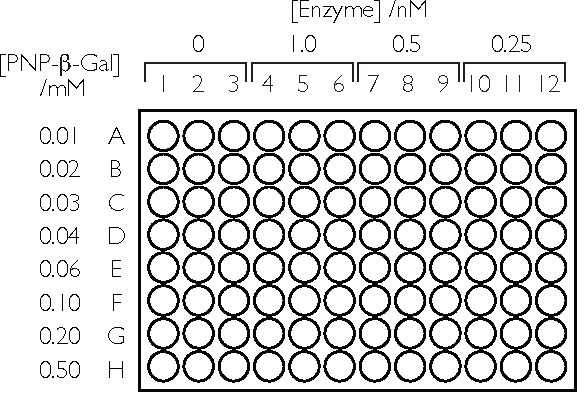
\includegraphics[scale=0.7]{Microtitreplateplan.pdf}
  \vspace{5mm}
  \label{fig:fig1}
\end{figure}

Two 96-well plates were set up. One contained the enzyme in phosphate buffer and the other PNP-\textbeta-D-Gal in a \qty{8}{\percent} mixture of isopropanol and phosphate buffer. The phosphate buffer had a concentration of \qty{0.100}{M} and was at pH 7.0. Volumes in each plate were equal. At time zero the contents of substrate plate was transferred to the enzyme plate by a multipipettor. The series of samples were prepared so that the final concentrations in the plate as described in the plate plan were realized.\sidenote[][-10mm]{Question: After the plates are mixed, what is the amount of isopropanol present in each sample? Do you think it will affect the results? Why did I choose to have a isopropanol as a small fraction of the solution?} The plate was placed in a plate reader and readings began 30~seconds after the addition of substrate. Absorbance was measured at \qty{405}{nm}.\sidenote[][0mm]{Question: What do we know about PNP-\textbeta-D-Gal that informed the choice of this wavelength.}

\section{Data Collection}

Data was exported from the plate reader as separate time/absorbance files names according to column and row. A python script to plot the initial results for each well in a column of the plate was used to produce the contact sheet of data below.

\begin{figure}[h!]

  \caption[0mm]{Plots of $A_{405}$ vs time for each well in the plate. Each column represents an experiment at eight different substrate concentrations. 
    
  \vspace{2mm}
  \noindent The \emph{Python} code for generating this plot is available via Google Colab.} 
 
  \vspace{-5mm}
    \centering
  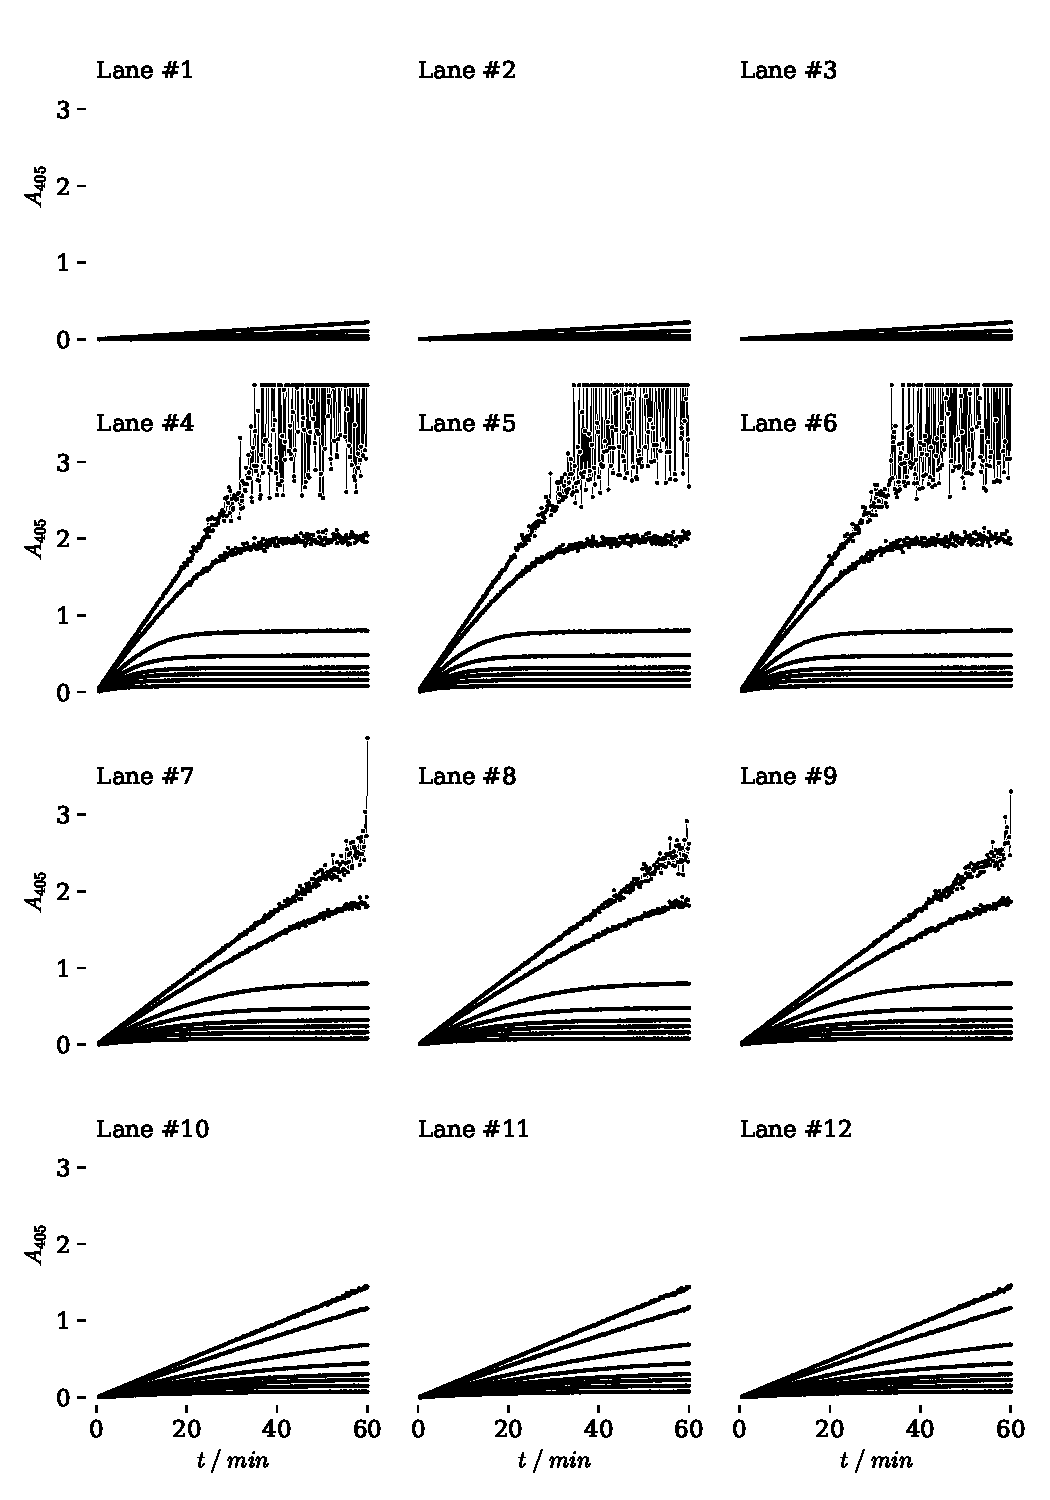
\includegraphics[scale=0.6]{contactsheetplotA.pdf}
  \vspace{2mm}
  \label{fig:fig2}
\end{figure}


\section{Observations}

Substantial experimental error was observed in the data and the measurements became unreliable when absorbances exceed the value of 2.\sidenote[][-0mm]{Question: The manufacturer of the plate reader advertised that precise readings could be obtained up to 3 absorbance units. Given what we know about how absorbance is calculated, please explain why the error is much greater at higher absorbance values.} 

The time frame of the experiment was such that most of the reactions reached completion. For initial rate analysis we must use the absorbance change in the few percent change in substrate concentration as the reaction proceeds. We want the slope to be as close as possible to the initial slope. I wrote a \emph{Python} script that plots data from a single well over a selected time frame, performing a linear fit of the data and calculating the residuals to confirm that we are using a time frame in which the data is mostly linear.  We want as much data as possible so would like a longer time frame, but we want to have little or no observable curve in the line as so want a small a time frame as possible after the start of the reaction. 

After examining many cells, I chose a time frame from zero to 3 minutes. This captures about 15 of the 358 data points collected over the hour duration of the experiment with no curvature detectable above the noise of random error.

\begin{figure}[h!]

  \caption[0mm]{Plots of $A_{405}$ vs time for well 7-B. [Enzyme] = \qty{0.5}{nM}, [PNP-\textbeta-D-Gal] = \qty{0.02}{mM}. Three time frames are show: the full \qty{60}{\minute}, \qty{12}{\minute}, and \qty{4}{\minute}. The residuals for the line fit of the \qty{4}{\minute} time frame are shown in the lower left plot. No curvature was detectable within the range of the experimental error.
  
  \vspace{2mm}
 \noindent The \emph{Python} code for generating this plot is available via Google Colab.} 
  \vspace{-0mm}
    \centering
  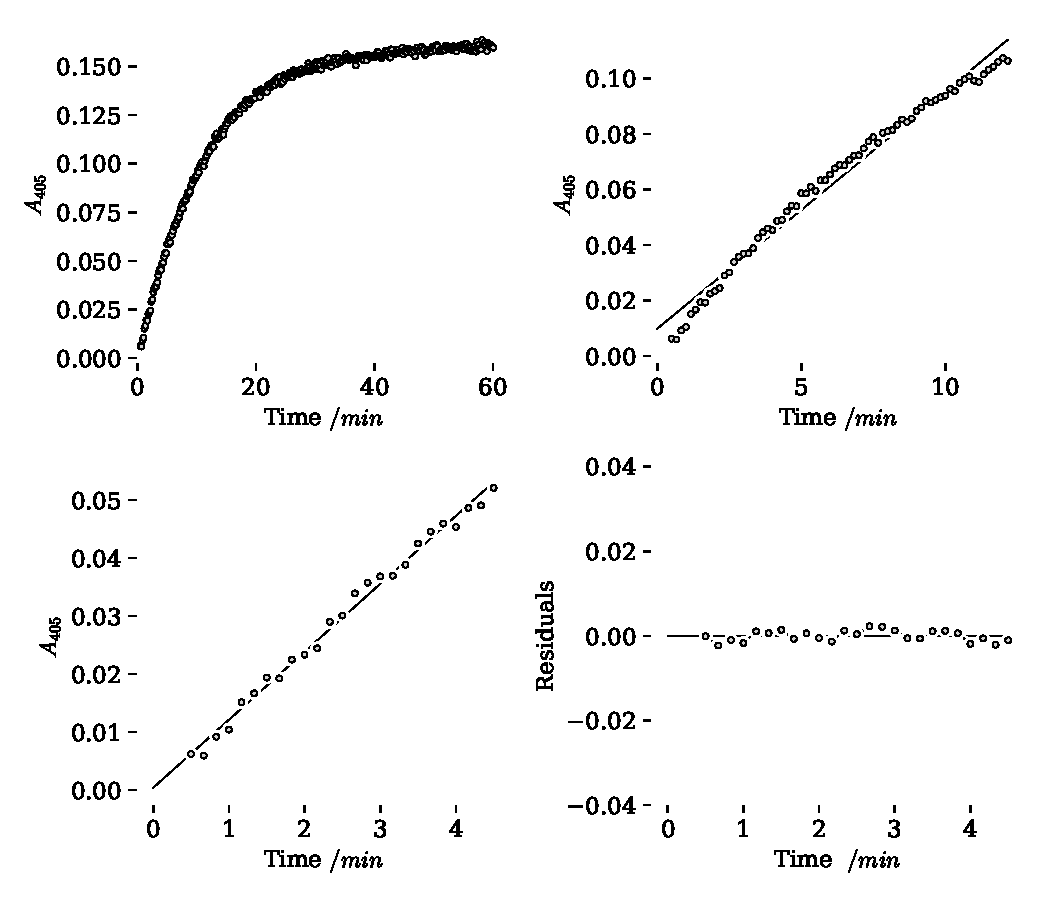
\includegraphics[scale=0.6]{Cell_w_residuals_7_B.pdf}
  \vspace{2mm}
  \label{fig:fig2}
\end{figure}



The short time frame was required because the highest enzyme con\-en\-tration resulted in reactions so rapid that substantial change in substrate concentration occurred in the first few moments. For wells where the sub\-strate concentration was at or below the \Km\ value, we saw significant curv\-a\-ture at beyond the shortest time frames. The diluted enzyme samples were linear over longer time frames and more data could have been used in these cases. I will use the short time frame discussed above to be consistent but future experiments with less enzyme may be able to use more data points before curvature is observed. Hopefully my unfortunate successor will find this information useful. The cake is a lie!

There is significant hydrolysis of the PNP-\textbeta-D-Gal in the absence of enzyme catalyst.  It is a very reactive molecule and at pH 7.0 the rate of hydrolysis is significant. It will be necessary to subtract the background rate from catalyzed rates to ensure accuracy.

\section{Data Analysis}

Based on the observations above I will create a \emph{Python} script to calculate the initial slope of absorbance change over time in each cell. We can calculate the rate of appearance of product using the molar extinction coefficient for phenolate anion and the $pK_a$ value for the phenol. The curve fit function will also report a standard deviation for the slope based on the random error in the data and the number of points. We will use this value as a measure of the precision of our data. The script will output the rate of reaction and the standard error for all 96 cells and save that data in a csv file.\sidenote[][0mm]{ The python code is available as an interactive \emph{Python} notebook via Google Colab.} 

Then I used another python script to plot the Michaelis-Menten plots using the rate data for each well that was output by the script described above. The script determines the mean value for each from the three exper\-i\-ments enzyme concentration. The background rate is subtracted and the resulting rate data with standard errors is plotted. using a curve fit to the Michaelis-Menten equation the \Vmax\ and \Km\ values are calculated. We know the enzyme concentration so we can calculate \kcat\ and $k_{cat}/K_M$ values.\sidenote[][0mm]{ The python code is available as an interactive \emph{Python} notebook via Google Colab.}

\section{Conclusion}

I have determined the $k_{cat}/K_M$ value for the native enzyme with the PNP-\textbeta-D-Gal substrate. The value with the lowest standard error was produced by the experiment with enzyme concentration set to \qty{0.25}{nM}. As a result, I will use this enzyme concentration in the subsequent survey of mutant \emph{\textbeta -galactosidases}

\section{Enzyme Survey} 

We now have a large library of purified \emph{\textbeta -galactosidases} from bacteria exposed to mutagens. many of these may contain no mutations, some many be inactive due to mutations in the active site and perhaps some will have a higher efficiency transglycosylation with the PNP-\textbeta-D-Gal substrate. Our synthesis goal seeks to manufacture a molecule that features the same phenol-\textbeta-galac\-tose group and we anticipate that the most efficient mutant for transferring the galactose to water will also be the most efficient for transferring it to a phenol.

I will set up plates with the following concentrations of PNP-\textbeta-D-Gal substrate in each lane: 0.005, 0.01, 0.015, 0.03, 0.06, 0.10, 0.20, 0.50 mM. In each column, we will have \qty{0.25}{nM} of a given mutant. One lane in each plate will be a control and contain no enzyme. This will give a background rate ofr the substrate hydrolysis. The experiment will then be carried out as above and the data collected as a set of csv files, one for each well.

\section{Analysis of Survey Data}

I have measured the absorbance vs. time of 12 plates. I will need to go to the lab where we make the mutants and get more samples. For some reason no one is answering the phone down there. brb.

\begin{quotation}This is where the last technical report written by your unfortunate predecessor ends. The data for the 12 plates of samples in the first survey attempt is included with this document. Please examine the data and use the \emph{Python} code that was created by your unfortunate predecessor to analyze the data and obtain $k_{cat}/K_M$ values for each enzyme in our library. Report your ten best candidates.

Be sure to reassure your excellent supervisors that you have found accurate values by presenting representative plots of initial rate data and Michaelis-Menten curves in your report. Show that you are confident that the time span that you chose to use will produce the best estimates of initial rate possible while also providing the maximum amount of data (and thus minimizing the standard error). Don't pick a number out of your hat for the time span. Investi\-gate your data and choose a value that will work best across the whole data set.

You have data sets for 1,152 wells to analyze. If you use \emph{Python} code to automate your data analysis then you might have time for that cake that you were promised.

Do not enter the microbiology lab. That area is currently closed for mainten\-ance.
\end{quotation}


\nobibliography{}

\end{document}